\documentclass{article}
\usepackage{amssymb, amsfonts}
\usepackage{fullpage}
\usepackage{enumerate}
\usepackage[linesnumbered,ruled,vlined]{algorithm2e}
\usepackage[usenames,dvipsnames]{xcolor}
\usepackage[colorlinks,allcolors=RoyalBlue]{hyperref}
\usepackage{enumitem}
\usepackage{graphicx} % Required for inserting images
\usepackage[margin=1in]{geometry}
\usepackage{xcolor}
\usepackage{amsmath}
\usepackage{tikz}
\usepackage{tkz-base}
\usepackage{tkz-euclide}
\usepackage{comment}

\usepackage[T1]{fontenc}
% \usepackage{palatino}
\usepackage{libertine, libertinust1math}
\usepackage{titlesec}
% \usepackage{newtxtext,newtxmath}
% \usepackage{kpfonts}

\renewcommand{\familydefault}{\sfdefault}
\renewcommand{\sfdefault}{LinuxLibertineT-TLF}


% For environments and alias
\usepackage{amsthm}
\usepackage{mdframed}
\usepackage{mathtools}
\usepackage{cleveref}
\newmdtheoremenv{assumption}{Assumption}

\DeclareMathOperator*{\argmin}{arg\,min}
\DeclareMathOperator*{\argmax}{arg\,max}
\newcommand{\loss}[1]{\mathcal{L}_\text{#1}}

\newcommand{\R}{\mathbb{R}}
\newcommand{\C}{\mathbb{C}}
\newcommand{\Z}{\mathbb{Z}}
\newcommand{\N}{\mathbb{N}}
\newcommand{\F}{\mathbb{F}}
\newcommand{\E}{\mathbb{E}}
\newcommand{\cO}{\mathcal{O}}
\newcommand{\ctO}{\Tilde{\cO}}
\newcommand{\mdot}{\:\cdot\:}
\newcommand{\jacf}{\nabla f}
\newcommand{\hesf}{\nabla^2 f}

\newcommand{\x}{\mathbf{x}}
\newcommand{\y}{\mathbf{y}}
\newcommand{\w}{\mathbf{w}}

\DeclarePairedDelimiter{\norm}{\lVert}{\rVert}
\DeclarePairedDelimiterX{\inner}[2]{\langle}{\rangle}{#1,#2}
\DeclarePairedDelimiter{\Set}{\lbrace}{\rbrace}
\DeclarePairedDelimiter{\abs}{|}{|}
\DeclarePairedDelimiter{\ceil}{\lceil}{\rceil}
\DeclarePairedDelimiter{\floor}{\lfloor}{\rfloor}
\DeclarePairedDelimiter{\paren}{(}{)}
\DeclarePairedDelimiter{\bracket}{[}{]}
\DeclarePairedDelimiter{\curly}{\lbrace}{\rbrace}
\DeclarePairedDelimiter{\card}{|}{|}
\DeclarePairedDelimiter{\norms}{\lVert}{\rVert^2}
\DeclarePairedDelimiter{\fnorm}{\lVert}{\rVert_F}
\DeclarePairedDelimiter{\infnorm}{\lVert}{\rVert_\infty}

\newcommand{\mincurly}[1]{\min\curly*{#1}}
\newcommand{\maxcurly}[1]{\max\curly*{#1}}
\newcommand{\Exv}[1]{\E\bracket*{#1}}
\newcommand{\bigO}[1]{\cO\paren*{#1}}
\newcommand{\bigtO}[1]{\ctO\paren*{#1}}
\newcommand{\prob}[1]{P\paren*{#1}}
\newcommand{\condprob}[2]{P\paren*{#1\mid#2}}

\newenvironment{solution}{
    \color{Red}
    \textbf{Solution:}
}

\title{CS 4782 Homework 1\vspace{-10pt}}
\author{Due: 2/12/26 11:59 PM on Gradescope}
\date{Late submissions accepted until 2/14/26 11:59 PM}

\begin{document}
    \maketitle \textbf{Note: For homework, you can work in teams of up to 2 people. Please include your teammates’ NetIDs and names on the front page and form a group on Gradescope. Grades are based on completion. Please attempt each problem and show your work.}

\section*{Problem 1: Backpropagation (30 points)}
\begin{enumerate}
\item (5) Suppose you have the following 3-layer fully connected neural network for a regression problem ($y \in \mathbb{R}^+$).

\begin{figure}[!ht]
    \centering
    \includegraphics[scale=0.6]{neural_net.jpg}
\end{figure}

We want to run \href{https://www.cs.cornell.edu/courses/cs4780/2018fa/lectures/lecturenote10.html}{empirical risk minimization} on this neural network using the MSE loss function, which for a single example $(x, y)$ is given by
$$L(\hat{y}, y) = (y - \hat{y})^2.$$\\
Assume that the activation function used, $\sigma(x)$, is $\texttt{ReLU}(x) = \texttt{max}(0, x)$. The following equations represent the forward pass through this neural network. Recall that the weights and bias of the $l^{th}$ layer can be written as $W^{[l]}$ and $b^{[l]}$ respectively. Here, $a^{[l]}$ denotes the pre-activation output of layer $l$ before applying ReLU, and $z^{[l]}$ denotes the post-activation output (the layer’s activation) after applying ReLU.

\begin{equation}
    \begin{split}
        z^{[0]} & = x\\
        a^{[1]} & = W^{[1]}z^{[0]} + b^{[1]}\\
        z^{[1]} & = ReLU(a^{[1]})\\
        a^{[2]} & = W^{[2]}z^{[1]} + b^{[2]}\\
        z^{[2]} & = ReLU(a^{[2]})\\
        a^{[3]} & = W^{[3]}z^{[2]} + b^{[3]}\\
        z^{[3]} & = ReLU(a^{[3]})\\
        \hat{y} & = z^{[3]}\\
    \end{split}
\end{equation}
Suppose we have the following training data point 
\[ \left( \begin{bmatrix}
	2 \\
	1 \\
    \end{bmatrix} , 10 \right) \]
and the weights and bias terms of our neural network are
\[ W^{[1]} = \begin{bmatrix}
	1 & 0 \\
	3 & 4 \\
	1 & 2
    \end{bmatrix}, \ 
 b^{[1]} = \begin{bmatrix}
	0  \\
       -2 \\
	5 
    \end{bmatrix}, \ \ \ 
W^{[2]} = \begin{bmatrix}
	2 & 6 & 1\\
	0 & 3 & 1
    \end{bmatrix}, \ 
 b^{[2]} = \begin{bmatrix}
	-23  \\
        -11 
    \end{bmatrix}, \ \ \
W^{[3]} = \begin{bmatrix}
	-2 & 3 \\
    \end{bmatrix}, \ 
 b^{[3]} = 18. \]
Calculate the values of each of the terms listed in equation (1) above.


\item (15) Using the backpropagation algorithm presented in Lecture 3, Slides 10-16, derive the sequence of terms derived during backpropagation to find gradients for this neural network, i.e. complete the following equations. You may use $ReLU'(x)$ to denote the gradient of the ReLU function. \\ \\

\makebox[\linewidth][l]{%
$
\begin{aligned}
\frac{\partial L}{\partial \hat{y}} &= \\
\frac{\partial L}{\partial z^{[3]}} &= \\
\frac{\partial L}{\partial a^{[3]}} &= \\[6pt]
\frac{\partial L}{\partial W^{[3]}} &= \\
\frac{\partial L}{\partial b^{[3]}} &= \\
\frac{\partial L}{\partial z^{[2]}} &= \\
\frac{\partial L}{\partial a^{[2]}} &= \\[6pt]
\frac{\partial L}{\partial W^{[2]}} &= \\
\frac{\partial L}{\partial b^{[2]}} &= \\
\frac{\partial L}{\partial z^{[1]}} &= \\
\frac{\partial L}{\partial a^{[1]}} &= \\[6pt]
\frac{\partial L}{\partial W^{[1]}} &= \\
\frac{\partial L}{\partial b^{[1]}} &= \\
\frac{\partial L}{\partial z^{[0]}} &= \\
\frac{\partial L}{\partial x} &=
\end{aligned}
$
}


\item (10) Given the same training point, weights, and bias terms as in part (a), calculate the gradients of each of the weights and bias terms.

\end{enumerate}

\section*{Problem 2: Efficiency of Random Hyperparameter Search (10 points)}

Hyperparameter search is an effective yet computationally expensive process in machine learning, particularly for small models. Let's say we are training a relatively large neural network that takes 2 minutes for each epoch, and we are training for 10 epochs.
We are interested in tuning the learning rate $\alpha\in[10^{-4}, 0.2]$, the L2 regularization strength parameter $\lambda_2\in[0, 100]$, and the dropout ratio $p\in[0, 0.2]$.

\begin{enumerate}
    \item (5) If we are doing Grid search with
    \begin{itemize}
        \item $\alpha=0.0001, 0.0005, 0.001, 0.002, 0.005, 0.01, 0.02, 0.05, 0.1, 0.2$ (10 values)
        \item $\lambda_2=0, 0.1, 1, 5, 10, 100$ (6 values)
        \item $p=0, 0.05, 0.1, 0.15, 0.2$ (5 values)
    \end{itemize}
    How many epochs in total are required to train all models to obtain the best performing set of hyperparameters?
    How long does it take?


    \item (5) Now let's assume that within the domain of $\alpha, \lambda_2, p$, there are 5\% of the combinations that can result in strong performance.
    Then for each trial of the training, we uniformly and independently sample the hyperparameters from their domain.
    How many trials do we need to run to have a high probability (95\%) that the search will find a strongly performing model? What if we want 99.5\% probability to find such a good hyperparameter setting?
\end{enumerate}

\section*{Problem 3: Optimization Methods (10 points)}

In class we saw several optimization methods. For each of the following techniques, explain its advantages over traditional gradient descent (approximately 3 sentences each). Note that $n > b > 1$.\\
\\Recall the update rule of Gradient Descent is \[
\w_{t+1}=\w_t-\alpha \frac{1}{n} \sum_{i=1}^{n} \nabla l(\w_t, \x_t).
\]

\vspace{1em}

\begin{enumerate}
    \item (3)
 Stochastic Gradient Descent
\[
\w_{t+1}=\w_t-\alpha\nabla l(\w_t, \x_t)
\]
\vspace{1.5em}
\item (3) Minibatch Stochastic Gradient Descent
\[
\w_{t+1} = \w_t - \alpha \frac{1}{b} \sum_{i=1}^{b} \nabla l(\w_t, \x_i)
\]
\vspace{1.5em}
\item (4) Stochastic Gradient Descent with Momentum
\[
m_{t+1} = \mu m_t - \alpha\nabla l(\w_t; \x_i)
\]

\[
\w_{t+1} = \w_t + m_{t+1}
\]


\vspace{1.5em}
\end{enumerate}



\maketitle

\section*{Problem 4: Convolutional Neural Networks (25 points)}
\begin{enumerate}
\item (4) Suppose you have a convolutional filter of size $3 \times 3$.  If you apply this filter to a grayscale image of size $36 \times 36$ with no padding and stride = 1, what is the dimension of the output? Show your work. \\


\item (4) Now suppose you apply \textit{two} filters of size $3 \times 3 \times 3$ on an RGB image of size $36 \times 36$ with padding = 3 and stride = 2, what are the dimensions of the output? Show your work. \\ 


\item (9) Derive a general formula for the output dimensions of a  convolutional operation. Suppose you have $l$ filters of size $k \times k \times c$ applied to an input image of size $n \times n \times c$ with stride $s$ and padding $p$, what is the dimension of the output? Explain the general formula you derive. \\

\item (8) Suppose you are given an $3 \times 3$ matrix from an image $I$ and a $2 \times 2$ convolutional kernel $K$. In the image matrix, each entry represents the grayscale color of a corresponding pixel.
	\[ I = \begin{bmatrix}
	6 & 0&  1 \\
	3 & 4 & 1 \\
	1 & 7 & 0
    \end{bmatrix} \]
and \[ K = \begin{bmatrix}
	   1 & 0 \\ 0 & -1
	   \end{bmatrix} \]
What is the output of applying the filter to the input with stride 1 without padding?\\

\vspace{3mm}
\end{enumerate}
\section*{Problem 5: Residual Networks (25 points)}
\begin{enumerate}
\item (5) What is the vanishing gradient problem in deep neural networks? Explain in approximately 3 sentences.\\


\item (3) Consider the following (plain) convolutional layers:

\begin{figure}[!ht]
    \centering
    \includegraphics[scale=0.5]{CNN_layers.png}
\end{figure}

Let $x$ be the input to the convolutions, $z_1$ and $z_2$ be the output of the 1st and second layers respectively, and $L$ be some loss function. You are given the following gradients:

$$ \frac{\partial L}{\partial z_2} = 0.01  $$
$$ \frac{\partial z_2}{\partial z_1} = 0.005  $$
$$ \frac{\partial z_1}{\partial x} = 0.1  $$

What is $\frac{\partial L}{\partial x}$? \\


\item (3) Now consider the following residual block:

\begin{figure}[!ht]
    \centering
    \includegraphics[scale=0.5]{ResBlock.png}
\end{figure}

Once again, let $x$ be the input to the convolutions, $z_1$ and $z_2$ be the output of the 1st and second layers respectively, $y = z_2 + x$ be the output of the residual block, and $L$ be some loss function. Assume the gradients are the same as in part 2(b), and that $\frac{\partial L}{\partial y} = 0.01$. What is $\frac{\partial L}{\partial x}$? \\


\item (4) Compare the gradients from parts (b) and (c). What do you notice? \\


\item (5) Suppose \textit{n} is the number of convolutional layers in a plain CNN. Let $x$ be the input to the convolutional layers, $z_i \in {\{z_1, z_2, ..., z_n\}}$ be the output of the $i$th convolutional layer, and $L$ be some loss function. You are given the following gradients:

$$\frac{\partial L}{\partial z_n} = 0.5$$
$$\frac{\partial z_i}{\partial z_{i-1}} = 0.5 \ \ \forall  \ 1 < i \leq n$$
$$\frac{\partial z_1}{\partial x} = 0.5$$

Graph $\frac{\partial L}{\partial x}$ as the number of layers $n$ increases from 1 to 6. 

\begin{center}
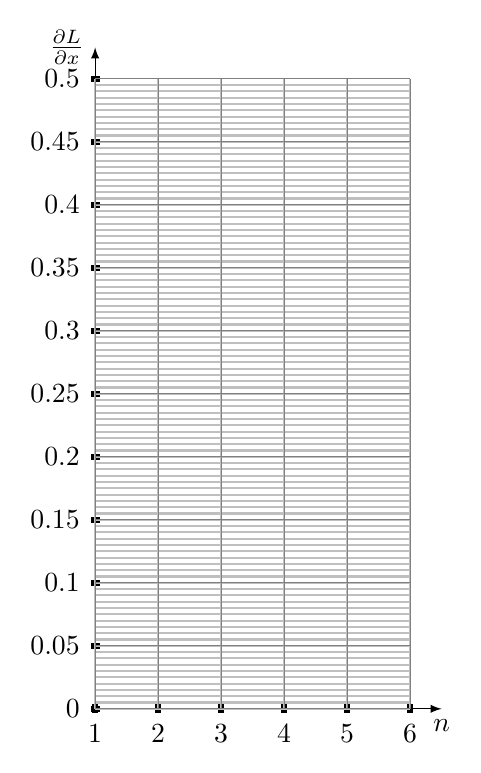
\begin{tikzpicture}[scale=0.8]
    \tkzInit[xmin=1,xmax=6,ymin=0,ymax=0.5, xstep=1, ystep=.05]
    \tkzGrid[sub,color=gray, subxstep=1.,subystep=.005]
    \tkzDrawX[label = $n$, tickwd = 2pt]
    \tkzLabelX[]
    \tkzDrawY[label = $\frac{\partial L}{\partial x}$, tickwd = 2pt]
    \tkzLabelY[]
    \tkzGrid
    \end{tikzpicture}
\end{center}

\item (5) Now suppose \textit{n} is the number of convolutional layers in a ResNet, in which a residual block consists of two convolutional layers. Again, let $x$ be the input to the convolutional layers, $z_i \in {\{z_1, z_2, ..., z_n\}}$ be the output of the $i$th convolutional layer, $y_j \in {\{y_1, y_2, ..., y_{n/2}\}}$ be the output of the $j$th residual block, and $L$ be some loss function. You are given the following gradients:

$$\frac{\partial L}{\partial y_{n/2}} = 0.5$$
$$\frac{\partial z_i}{\partial y_{i-2}} = 0.5 \ \ \forall  \ 1 < i \leq n$$
$$\frac{\partial z_i}{\partial z_{i-1}} = 0.5 \ \ \forall  \ 1 < i \leq n$$
$$\frac{\partial z_1}{\partial x} = 0.5$$

Graph $\frac{\partial L}{\partial x}$ as the number of layers $n$ increases from 2 to 6 (i.e. the number of residual blocks increases from 1 to 3). Note you only need to plot points where $n$ is even.

\begin{center}
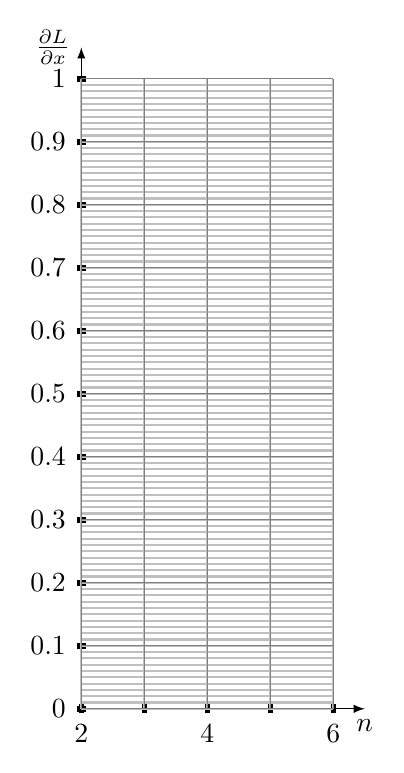
\begin{tikzpicture}[scale=0.8]
    \tkzInit[xmin=2,xmax=6,ymin=0,ymax=1, xstep=1, ystep=.1]
    \tkzGrid[sub,color=gray, subxstep=1.,subystep=.01]
    \tkzDrawX[label = $n$, tickwd = 2pt]
    \tkzLabelX[step = 2]
    \tkzDrawY[label = $\frac{\partial L}{\partial x}$, tickwd = 2pt]
    \tkzLabelY[]
    \tkzGrid
    \end{tikzpicture}
\end{center}
\end{enumerate}

\end{document}